% !TeX root = ../../thesis.tex

\section{\acf{PI}}

\subsection{Boot Sequence}

% https://edk2-docs.gitbook.io/edk-ii-build-specification/2_design_discussion/23_boot_sequence

focus will be on dxe and transient system load
\autoref{fig:pi-phases}



\begin{figure}[htb]%
    \centering%
    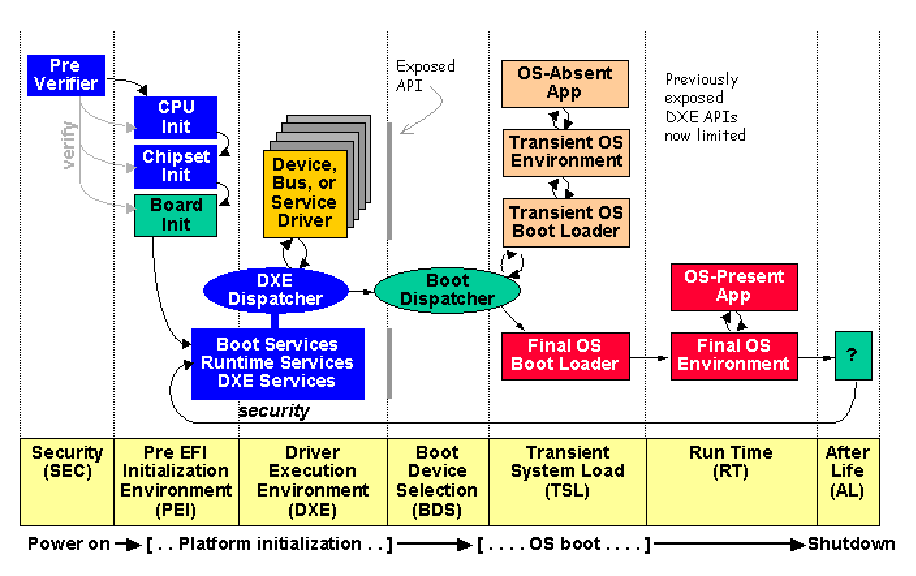
\includegraphics[width=\textwidth]{pi_boot_sequence}%
    \caption{\ac{PI} Architecture Firmware Phases \cite[Figure 2-1]{pi-spec}}%
    \label{fig:pi-phases}%
\end{figure}


\begin{enumerate}
    \item{\acf{SEC}}
    The Security phase is the first code executed by the CPU, it is uncompressed and executed directly from flash. It consists of platform specific assembly.

    \begin{itemize}
        \item  Handles all platform restart events (power on, wakup from sleep, etc)
        \item  Creates a temporary memory state by configuring the CPU Cache as RAM (CAR) no evictions mode
        \item  Serves as the root of trust in the system
        \item  Passes handoff information to the Pre-EFI Initialization (PEI) Foundation
    \end{itemize}


    % Since the CPU doesn't know about UEFI or BIOS the initial step is exactly the same, it starts in 16-bit real mode and fetches it's first instruction from `CS = 0xF000` and `IP = 0xFFF0` but instead of shifting `CS` left by four bits and adding `IP`, the `CS` base register is initialized to `0xFFFF'0000`. So the first instruction is fetched from the physical address `0xFFFF'FFF0` (`0xFFFF'0000 + 0xFFF0`). The CS base address remains at this initial value until the CS selector register is loaded by software (e.g. far jump or call instruction)

    \begin{itemize}
        \item Populates Reset Vector Data structure
        \item Saves Built-in self-test (BIST) status
        \item Enables protected mode (16 bit -> 32 bit)
        \item Configures temporary RAM (not only limited in processor cache) by using MTRR to configure CAR.
    \end{itemize}

    Passing of handoff information to the PEI phase:

    \lstinline{typedef VOID EFIAPI (*EFI_PEI_CORE_ENTRY_POINT)(IN CONST EFI_SEC_PEI_HAND_OFF *SecCoreData, IN CONST EFI_PEI_PPI_DESCRIPTOR *PpiList);}

    SEC Core Data:
    \begin{itemize}
        \item Points to a data structure containing information about the operating environment:
        \item Location and size of the temporary RAM
        \item Location of the stack (in temporary RAM)
        \item Location of the Boot Firmware Volume (BFV)
    \end{itemize}


    PPI list:
    \begin{itemize}

        \item Temporary RAM support PPI

              An optional service that moves temporary RAM contents to permanent RAM.

        \item SEC platform information PPI

              An optional service that abstracts platform-specific information to locate the PEIM dispatch order and maximum stack capabilities.
    \end{itemize}


    % The SEC phase is the first phase in the UEFI boot process. It is specified in \cite[Vol 1, Section 13 ]{pi-spec}. Under its responsibilities fall setting up temporary memory used for the stack and the establishment of the system's root of trust which is a foundation for all secure operations. Inductive security designs rely on this root of trust to build a chain of trust by having a module verify the integrity of its subsequent module.
    ref to PSP

    inductive security design
    integrity of next module checked by the previous module

    handles all platform restart events
    applying power to system from unpowered state
    restarting from active state
    receiving exception conditions

    creates temporary memory store
    possibly CPU \ac{CAR}
    cache behaves as linear store of memory
    no evictions mode
    every memory access is a hit
    eviction not supported as main memory is not set up yet and would lead to platform failure


    final step
    Pass handoff information to the \ac{PEI} Foundation
    % what is the PEI foundation
    \begin{itemize}
        \item state of platform
        \item location and size of the \ac{BFV}
        \item location and size of the temporary RAM
        \item location and size of the stack
        \item optionally one or more \acp{HOB} via the \ac{SEC} \ac{HOB} Data \ac{PPI}
    \end{itemize}


    Part of this process is a so called \ac{HOB} with a function pointer to a procedure to verify PE modules.

    SEC Platform Information PPI
    information about the health of the processor

    SEC HOB Data PPI

    \item{\acf{PEI}}
    Configures a system meeting the minimum prerequisites for the Driver Execution (DXE) phase, which is generally a linear array of RAM large enough for successful execution.

    PEI provides a framework allowing vendors to supply initialization modules for each functionally distinct piece of system hardware which must be initialized before the DXE phase.

    PEI design goals of the PI architecture:
    \begin{itemize}
        \item Maintenance of the chain of trust, includes protection and authorization of PEI modules
        \item Provide a core PEI module
        \item Independent developement of intialization modules
    \end{itemize}
    The PEI phase consists of the PEI Foundation core and specialized plug-ins known as Pre-EFI Initialization Modules (PEIMs).

    Since the PEI phase is very early in the boot process it can't assume reasonable amounts of RAM so the features are limited:
    \begin{itemize}
        \item Locating, validating and dispatching PEIMs
        \item Communication between PEIMs
        \item Providing Hand-Off Data for DXE phase
        \item Initializing some permanent memory complement
        \item Describing the memory in Hand-Off Blocks (HOBs)
        \item Describing the firmware volume locations in HOBs
        \item Passing control into the Driver Execution Environment (DXE) phase
        \item Discover boot mode and possibly resume from sleep state
    \end{itemize}
    PEI Service Table visible to all PEIMs in the system, a pointer to this table is passed as an argument via the PEIM entry point, it is also part of each PEIM-to-PEIM Interface (PPI).


    % | Service                  | Description                                                                                                                                 |
    % | ------------------------ | ------------------------------------------------------------------------------------------------------------------------------------------- |
    % | PPI Services             | Manages PPIs to facilitate intermodule calls between PEIMs. Interfaces are installed and tracked on a database maintained in temporary RAM. |
    % | Boot Mode Services       | Manages the boot mode (S3, S5, normal boot, diagnostics, etc.) of the system                                                                |
    % | HOB Services             | Creates data structures called Hand-Off Blocks (HOBs) that are used to pass information to the next phase of the PI Architecture.           |
    % | Firmware Volume Services | Finds PEIMs and other firmware files in the firmware volumes                                                                                |
    % | PEI Memory Services      | Provides a collection of memory management services for use both before and after permanent memory has been discovered                      |
    % | Status Code Services     | Provides common progress and error code reporting services (for example, port 080h or a serial port for simple text output for debug).      |
    % | Reset Services           | Provides a common means by which to initiate a warm or cold restart of the system.                                                          |

    % #### PEI Foundation/Core

    PEI Foundation code is portable across all platforms of a given instruction-set. The set of exposed services is the same across different microarchitextures and allows PEIMs to be written in C.

    - Dispatches PEIMs
    - Maintains boot mode
    - Initializes permanent memory
    - Invokes DXE loader

    % #### PEI Dispatcher

    The PEI Dispatcher evaluates dependencies of PEIMs in the firmware volume, these dependencies are PPIs. The Dispatcher holds internal state machines to check dependencies of PEIMs, it starts executing PEIMs whose dependencies are statisfied to build up dependencies of other PEIMs, this is done until the dispatcher cannot invoke any more PEIMs. Then the DXE Initial Program Loader (IPL) PPI is invoked to pass control to the DXE phase.

    % #### Pre-EFI Initialization Modules (PEIMs)
    PEIMs are specialized drivers that personalize the PEI Foundation to the platform. They are analogus to DXE driver and generally correspond to the components being initialized. It is strongly recommended that PEIMS do only the minimum necessary work to initialize the system to a state that meets the prerequisites of the DXE phase. PEIMs reside in firmware volumes (FVs).

    % #### PEIM-to-PEIM Interfaces (PPIs)
    PEIMs communicate with each other using a structure called PPI. A PPI is a GUID pointer pair. The GUID is used to identifiy a certain service and the pointer provides access to data structures and services of the PPI.

    % There are two kinds of PPIs:
    % - Architectural PPIs
    % - Additional PPIs

    An architectural PPI is described in the PEI Core Interface Specification (CIS) and the GUID is known to the PEI Foundation. They typically provide a common interface to the PEI Foundation to a service with platform specific implementation.

    An additional PPI is important for interoperability but isn't required by the PEI Foundation, they can be classified as mandatory or optional.


    \begin{itemize}
        \item init permanent memory
        \item describe memory in \acp{HOB}
        \item describe \ac{FV} in \acp{HOB}
        \item pass control to \ac{DXE}
    \end{itemize}

    crisis recovery (what is this?)
    resuming from S3 sleep state
    linear array of RAM
    \ac{PEIM} provides a framework to allow vendors to supply separate initialization modules for
    each functionally distinct piece of system hardware that must be initialized prior to the DXE phase \cite{pi-spec}

    % design goals
    maintenance of chain of trust, protection against unauthorized updates to the PEI phase or modules
    authentication of the PEI Foundation and its modules
    provide core PEI module (PEI foundation) processor architecture independent, supports add-in moudles from vendors for processors, chipsets, RAM

    % what it does
    Locating, validating, and dispatching PEIMs
    Facilitating communication between PEIMs
    Providing handoff data to subsequent phases

    \item{\acf{DXE}}


    % - DXE Foundation/Core
    % - DXE Dispatcher
    % - DXE Drivers

    % #### DXE Foundation

    The DXE Foundation produces a set of Boot, Runtime and DXE Services and exposes them through handle databases in the EFI System Table. It is designed to be completely portable, independent of processor, chipset and platform. The only dependent of the Hand-Off Blocks from the PEI phase, after these are processed the all prior phases can be unloaded.

    % #### DXE Dispatcher

    The DXE Dispatcher discovers DXE drivers within the Firmware Volume (FV) and executes them in the correct order, respecting their dependencies towards each other. The Firmware Volume file format allows the DXE driver images to be packaged with expressions about their dependencies. Since the DXE Drivers are PE/COFF images the dispatcher comes with an apropriate loader to load and execute the image format.

    % #### DXE Drivers

    % - Drivers that execute very early in the DXE phase
    % - Drivers that comply with the UEFI Driver Model

    The DXE Drivers are responsible for initializing the processor, chipset,
    and platform components as well as providing software abstractions for console and
    boot devices in the form of services.

    dxe core/foundation
    platform independent
    is implementation of UEFI
    UEFI Boot Services
    UEFI Runtime Services
    DXE Services

    dxe dispatcher
    discover drivers stored in firmware volumes and execute in proper order
    apriori file optionally in FV or depex of driver
    after dispatching all drivers in the dispatch queue hands control over to BDS

    dxe drivers
    init processor, chipset and platform
    produce arichtectural protocols and \ac{I/O} abstractions for consoles and boot devices

    % responsibilities
    initializing the processor, chipset, and platform components
    providing software abstractions for system services, console devices, and boot devices.

    \item{\acf{BDS}}
    The DXE Foundation will hand control to the BDS Architectural Protocol after all of the DXE drivers whose dependencies have been satisfied have been loaded and executed by the DXE Dispatcher.

    % - Initializing console devices based on the ConIn, ConOut, and StdErr environment variables
    % - Loading device drivers listed in the DriverOrder environment variables
    % - Attempting to load and execute boot selections list from the BootOrder environment variables

    During the BDS phase new Firmware Volumes (FV) might be discovered and control is once again handed to the DXE Dispatcher to load drivers found on these additional volumes.


    DXE arichtectural protocol
    one function entry
    platform boot

    attempts to connect boot devices required to load the os
    discovers volumes containing new drivers
    calls DXE dispatcher
    doesnt return when successfully booting OS

    UEFI itself only specifies the NVRAM variables used in selecting boot options
    leaves the implementation of the menu system as value added implementation space \cite{uefi-spec}

    \cite{pi-spec}

    \begin{itemize}
        \item Initializing console devices
        \item Loading device drivers
        \item Attempting to load and execute boot selections
    \end{itemize}

    \item{\acf{TSL}}

    The Transient System Load (TSL) is primarily the OS vendor provided boot loader. Both the TSL and the Runtime Services (RT) phases may allow access to persistent content, via UEFI drivers and UEFI applications. Drivers in this category include PCI Option ROMs.

    This phase ends when an OS boot loader calls 'ExitBootServices()'.

    boottime and runtime services/driver
    bootloader
    \cite[13.3 System Partition]{uefi-spec}
    \cite[3.5.1.1]{uefi-spec}

    ExitBootServices()

    \item{\acf{RT}}
    Boot service drivers have been unloaded and only runtime services are accessible.


    runtime services/driver

    \item{\acf{AL}}
    The After Life (AL) phase consists of persistent UEFI drivers used for storing the state of the system during the OS orderly shutdown, sleep, hibernate or restart processes.

    hibernation
    sleep

\end{enumerate}

\subsection{\acs{UEFI}/\acs{PI} Firmware Images}

Firmware Images are stored in Flash Devices (FD), a Firmware Volume (FV) serves as file level interface. Usually multiple FVs are present in a single FD but a signle FV can also be distributed via multiple FDs.
A FV is formatted with a binary file system, typically with Firmware File System (FFS).

In a FFS modules are stored as files, they can be executed at the fixed address from Read Only Memory (ROM) or through relocation in loaded memory. Within a file are multiple sections which then contain the "leaf" images. These are for example PE32 images.

% https://edk2-docs.gitbook.io/edk-ii-build-specification/2_design_discussion/22_uefipi_firmware_images
\cite[Volume 3, 2.1]{pi-spec}

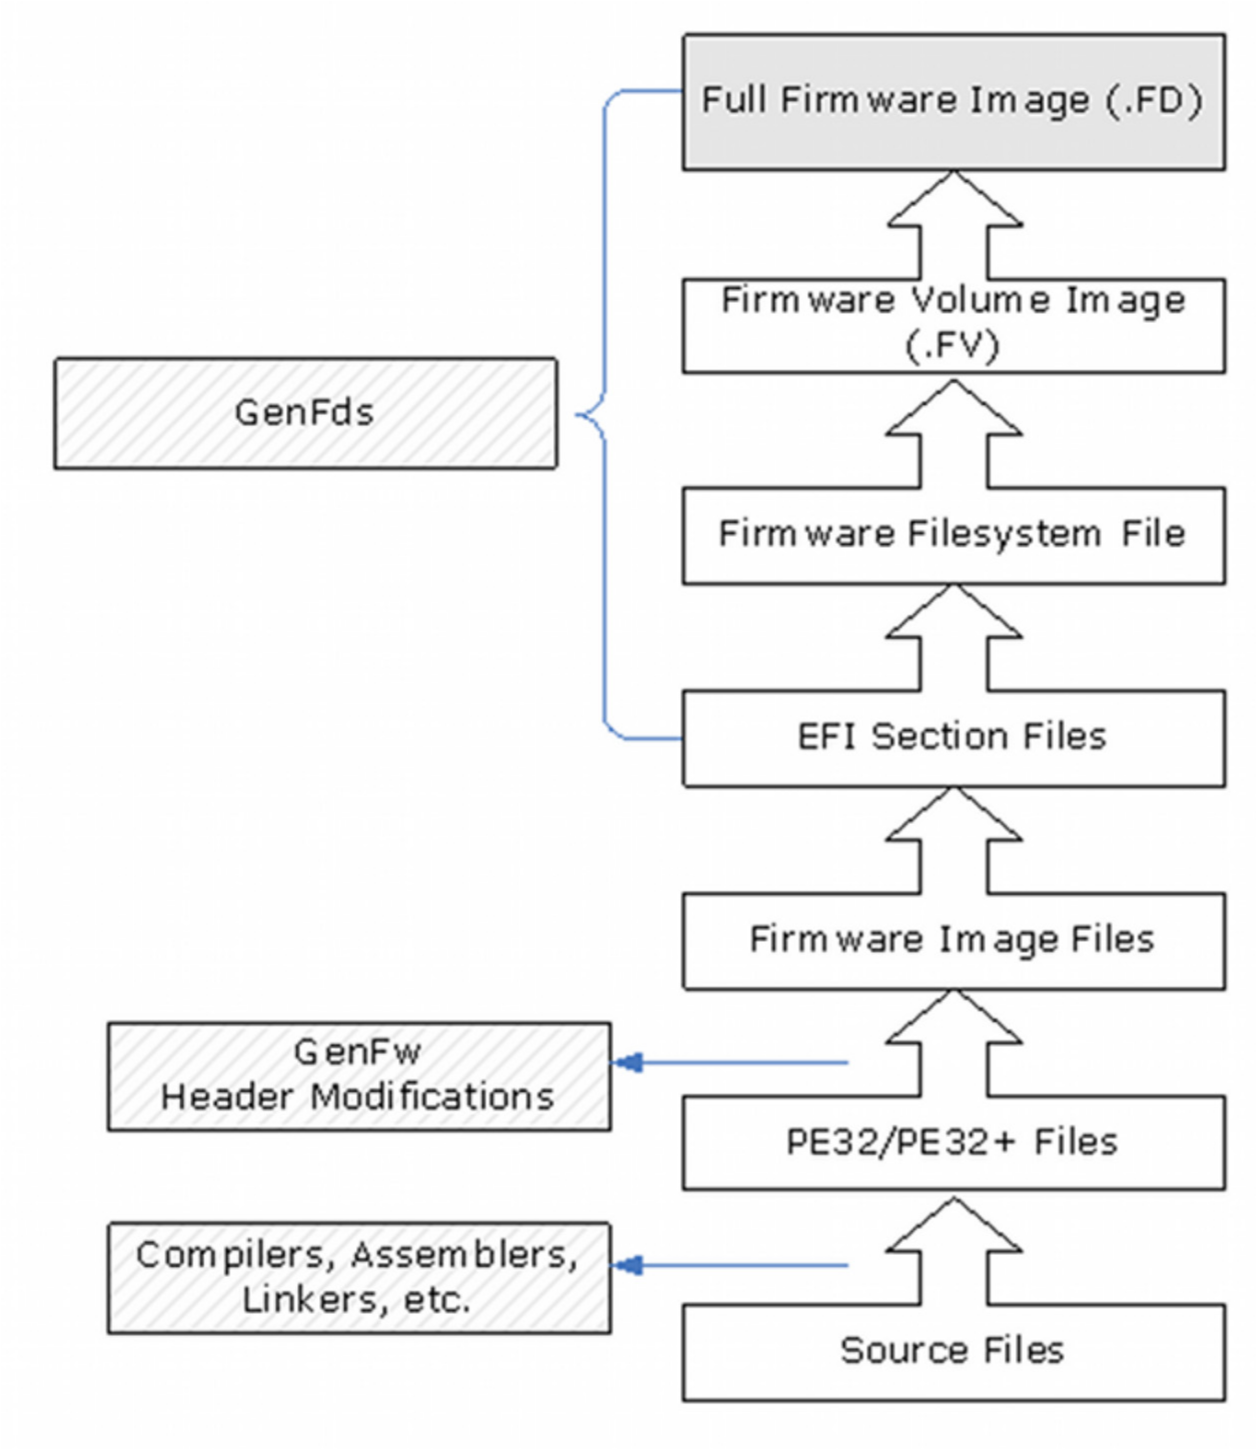
\includegraphics[width=\textwidth]{flash_device}
\ac{FD}
persistent
physical device
contains firmware code and/or data
typically flash
may be divided into smaller pieces to form multiple logical firmware devices
multiple physical firmware devices may be aggregated into one larger logical firmware device

\acf{FV}
logical device
organized into a file system
attributes such as
- size
- formatting
- read/write access

\acf{FFS}
organization of files and free space
no dierectory hierarchy
all files flat in root dir
parsing requires walking for beginning to end

firmware files
types
% PEI_CORE
% PEIM
% DXE_CORE
% DRIVER
% FIRMWARE_VOLUME_IMAGE
% FREEFORM

some file types are sub-divided in file sections

file sections can be either
encapsulation or leaf
leaf sections such as
PE32
% DXE_DEPEX
% PEI_DEPEX
RAW
VERSION
TE

dxe drivers files
contain one PE32 executable section
may contain version section
may contain dxe depex section

freeform files
can contain any combination of sections

PEI phase Service Table
FfsFindNextFile, FfsFindFileByName and FfsGetFileInfo

DXE phase
% EFI_FIRMWARE_VOLUME2_PROTOCOL

depex

\cite{tianocore-edk2-build-spec}

% !TeX root = ../../thesis.tex

\subsection{Security}
\label{sec:uefi-pi:pi:security}

The \ac{PI} specification defines \acp{PPI} and \ac{DXE} protocols which can be used to validate images when loading them.
During the \ac{PEI} phase, the \emph{\ac{PEI} Guided Section Extraction \ac{PPI}} can be used to authenticate file sections, while the \emph{Security \ac{PPI}} implements the policy response to the authentication result.
The \ac{DXE} phase has counter parts in the form of the \emph{Guided Section Extraction Protocol} and the \emph{Security Architectural Protocol}.
The policy response may be the locking of flash upon authentication failure or attestation logging \cite[Vol. 2, Section 12.9.1]{pi-spec}.
It also has the architectural protocol \emph{Security2 Architectural Protocol}, which implements Secure Boot validation, \ac{TCG} measured boot, and User Identity policy for image loading.
The implementation of the boot service \code{LoadImage()} has to use these protocols in accordance to the rules defined in \cite[Vol. 2, Section 12.9.2]{pi-spec}.
The Security2 protocol is invoked on every loaded image, with the Security protocol being invoked afterwards on images loaded through the Firmware Volume Protocol.
When the Security2 protocol is not installed it uses the Security protocol regardless of the image's origin.

\subsubsection{Hardware Validated Boot}

Secure Boot relies on the firmware as its root of trust.
Hardware validated boot is able to shift the root of trust out of the firmware image into a smaller part in the hardware, in hopes to reduce the size of the attack vector.
This part performs validation of the \ac{IBB} before handing over execution to the firmware image \cite{tianocore-understanding-uefi-secure-boot-chain}.

\subsubsection{Firmware Protection}

The \ac{PI} specification defines an \emph{End of \acs{DXE} Event}, which indicates the introduction of third party software execution to the platform.
Up until this point it is assumed that the entire system software is under the control of the platform manufacturer.
Drivers may react to this event by locking critical system resources, using the \ac{SMM} related services \cite[Vol. 2, 5.1.2.1]{pi-spec}.
The \ac{SMM} is a secure execution environment, achieved by isolation from the rest of the system, through the \ac{CPU} \cite[Vol. 4, Section 1.3]{pi-spec}.
The \ac{PI} reference implementation also makes use of this event to lock the device that stores the firmware image \cite{tianocore-edk2-fmpdxe}.

